\documentclass{article}
\usepackage[margin=1in]{geometry}
\usepackage{tikz}
\usetikzlibrary{positioning}
\usepackage{tcolorbox}
\usepackage{fontawesome5}
\usepackage{skak}
\usepackage{xcolor}

% Define benchmark command
\newcommand{\benchmark}{ChemChain}

\begin{document}

\begin{figure}[t]
    \centering

    % Chemistry problem with visual chain
    \begin{tcolorbox}[
        title=\textbf{Chemistry: Reaction Cascade} \hfill {\small\colorbox{teal!20}{Medium} \quad 9 steps},
        colframe=teal!70!black,
        colback=teal!3,
        boxrule=0.8pt,
        width=\textwidth
    ]
    \small
    \begin{tikzpicture}[remember picture, overlay]
        \node[opacity=0.08, anchor=east] at ([xshift=-0.3cm, yshift=0cm]current page.east) {\Huge\faFlask};
    \end{tikzpicture}

    \textbf{Dependency graph:}
    \begin{center}
    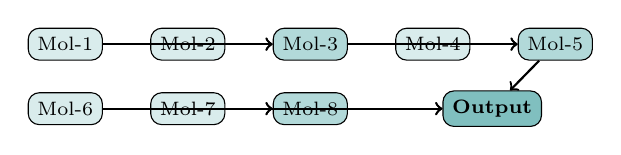
\begin{tikzpicture}[node distance=0.6cm, every node/.style={font=\scriptsize}]
        \node[draw, rounded corners, fill=teal!15] (m1) {Mol-1};
        \node[draw, rounded corners, fill=teal!15, right=of m1] (m2) {Mol-2};
        \node[draw, rounded corners, fill=teal!30, right=of m2] (m3) {Mol-3};
        \node[draw, rounded corners, fill=teal!15, right=of m3] (m4) {Mol-4};
        \node[draw, rounded corners, fill=teal!30, right=of m4] (m5) {Mol-5};
        \node[draw, rounded corners, fill=teal!15, below=0.4cm of m1] (m6) {Mol-6};
        \node[draw, rounded corners, fill=teal!15, right=of m6] (m7) {Mol-7};
        \node[draw, rounded corners, fill=teal!30, right=of m7] (m8) {Mol-8};
        \node[draw, rounded corners, fill=teal!50, right=1.2cm of m8] (out) {\textbf{Output}};

        \draw[->, thick] (m1) -- (m3);
        \draw[->, thick] (m2) -- (m3);
        \draw[->, thick] (m3) -- (m5);
        \draw[->, thick] (m4) -- (m5);
        \draw[->, thick] (m6) -- (m8);
        \draw[->, thick] (m7) -- (m8);
        \draw[->, thick] (m5) -- (out);
        \draw[->, thick] (m7) -- (out);
        \draw[->, thick] (m8) -- (out);
    \end{tikzpicture}
    \end{center}

    \vspace{-0.3cm}
    \begin{tabular}{@{}p{0.48\textwidth}p{0.48\textwidth}@{}}
    \textit{Sample step (Subproblem 3):} React Mol-1 + Mol-2 in THF at room temp. Predict major product. &
    \textit{Final step:} Count hydrogens in Mol-5, Mol-7, Mol-8. \\
    \end{tabular}

    \vspace{0.2cm}
    \hfill \textbf{Answer:} \texttt{[19, 15, 23]}
    \end{tcolorbox}

    \vspace{0.3cm}

    % Two-column for Chess and Math
    \begin{minipage}{0.48\textwidth}
        \begin{tcolorbox}[
            title=\textbf{Chess: Minimax Search} \hfill {\small\colorbox{orange!20}{Easy}},
            colframe=orange!70!black,
            colback=orange!3,
            boxrule=0.8pt
        ]
        \footnotesize

        \begin{center}
        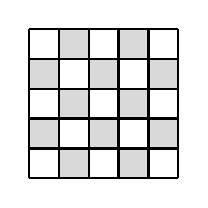
\begin{tikzpicture}[scale=0.38]
            % Draw 5x5 board
            \foreach \x in {0,...,4} {
                \foreach \y in {0,...,4} {
                    \pgfmathparse{mod(\x+\y,2) ? "gray!30" : "white"}
                    \fill[\pgfmathresult] (\x,\y) rectangle (\x+1,\y+1);
                }
            }
            \draw[thick] (0,0) grid (5,5);
            % Knight at (0,4)
            \node at (0.5,4.5) {\small$\symknight$};
            % Pawns
            \node at (2.5,4.5) {\small$\sympawn$};
            \node at (3.5,2.5) {\small$\sympawn$};
            \node at (1.5,1.5) {\small$\sympawn$};
        \end{tikzpicture}
        \end{center}

        \vspace{-0.2cm}
        Alice (max) and Bob (min) alternate capturing pawns with the knight. Each capture uses minimum moves. Find max total moves under optimal play.

        \vspace{0.2cm}
        \textit{Requires:} BFS + minimax over $3!$ orderings

        \vspace{0.2cm}
        \hfill \textbf{Answer:} [Redacted]
        \end{tcolorbox}
    \end{minipage}%
    \hfill%
    \begin{minipage}{0.50\textwidth}
        \begin{tcolorbox}[
            title=\textbf{Math: Dependent Problem Chain} \hfill {\small\colorbox{violet!20}{6 nodes}},
            colframe=violet!70!black,
            colback=violet!3,
            boxrule=0.8pt
        ]
        \footnotesize

        \begin{center}
        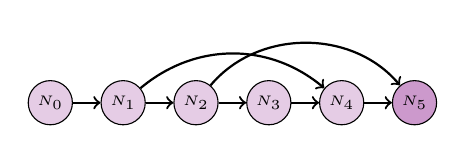
\begin{tikzpicture}[node distance=0.35cm, every node/.style={font=\tiny, inner sep=2pt}]
            \node[draw, circle, fill=violet!20] (n0) {$N_0$};
            \node[draw, circle, fill=violet!20, right=of n0] (n1) {$N_1$};
            \node[draw, circle, fill=violet!20, right=of n1] (n2) {$N_2$};
            \node[draw, circle, fill=violet!20, right=of n2] (n3) {$N_3$};
            \node[draw, circle, fill=violet!20, right=of n3] (n4) {$N_4$};
            \node[draw, circle, fill=violet!40, right=of n4] (n5) {$N_5$};
            \draw[->, thick] (n0) -- (n1);
            \draw[->, thick] (n1) -- (n2);
            \draw[->, thick] (n2) -- (n3);
            \draw[->, thick] (n3) -- (n4);
            \draw[->, thick] (n4) -- (n5);
            \draw[->, thick, bend left=40] (n1) to (n4);
            \draw[->, thick, bend left=50] (n2) to (n5);
        \end{tikzpicture}
        \end{center}

        \vspace{-0.1cm}
        \renewcommand{\arraystretch}{1.1}
        \begin{tabular}{@{}r@{: }p{5.8cm}@{}}
        $N_0$ & Guessing game strategies (59 values, 5 guesses) \\
        $N_1$ & Triangle area product ($RL = N_0 - 36428$) \\
        $\vdots$ & \textit{Each node transforms prior answers} \\
        $N_5$ & Block-splitting expected value \\
        \end{tabular}

        \vspace{0.2cm}
        \hfill \textbf{Answer:} [Redacted]
        \end{tcolorbox}
    \end{minipage}

    \caption{\textbf{\benchmark} problems require compositional reasoning: solving intermediate subproblems whose outputs feed downstream steps. \colorbox{teal!15}{Selection steps} identify molecules/values; \colorbox{teal!35}{reaction steps} combine them. Chains span 6--9 nodes and thousands of reasoning tokens.}
    \label{fig:sample-problems}
\end{figure}

\end{document}
